\section{Chapter 4: Fusion on Earth}

\subsection{Write equations and explain similarities and differences between fusion reactions that are realistically possible to do on earth.}
\solutionblock{Different reaction types: 
\begin{enumerate}
    \item D-T: \ch{D} + \ch{T} $\rightarrow$ \ch{^{4}He} + \ch{n} + 17.6 MeV
    \item D-D: \ch{D} + \ch{D} $\rightarrow$ \ch{^{3}He} + \ch{n} + 3.3 MeV
    \item D-D: \ch{D} + \ch{D} $\rightarrow$ \ch{T} + \ch{p} + 4.0 MeV
    \item D-Helium-3: \ch{D} + \ch{^{3}He} $\rightarrow$ \ch{^{4}He} + \ch{p} + 18.3 MeV
\end{enumerate}
The D-T reaction has the highest cross-section and can be accomplished with the lowest temperatures. The D-D reaction is the more difficult to achieve but doesn't require Tritium. Nevertheless, the most realistic to achieve is the D-T reaction.\\
}


\subsection{Why is tritium a scarce resource and how to produce it?}
\solutionblock{Because tritium is a radioactive isotope of Hydrogen with a half-life of 12.3 years. It is produced in the upper atmosphere by cosmic rays. Other than that there are no significant natural sources of tritium.\\
Tritium is therefore produced by irradiating Lithium-6 or Lithium-7 with neutrons: 
\begin{enumerate}
    \renewcommand\labelenumi{} 
    \item \ch{^{6}Li} + \ch{n} $\rightarrow$ \ch{T} + \ch{^{4}He} + 4.8 MeV
    \item \ch{^{7}Li} + \ch{n} $\rightarrow$ \ch{T} + \ch{^{4}He} + \ch{n} - 2.5 MeV
\end{enumerate}
Some would even be produced inside a fusion reactor by the D-D reaction.\\
}

\subsection{Draw the overall fuel cycle of a D-T fusion plant.}
\solutionblock{
    \begin{figure}[H]
        \centering
        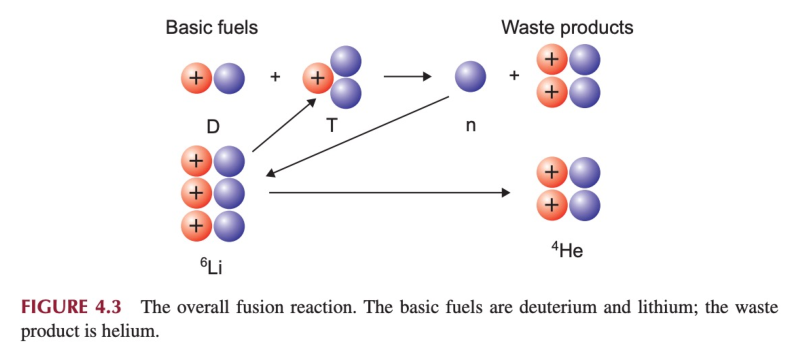
\includegraphics[width=0.75\textwidth]{chapters/fig/4_fuel_cycle.png}
        \caption{Fuel Cycle of a D-T Fusion Plant}
        \label{fig:4_fuel_cycle}
    \end{figure}
}

\subsection{Explain the difficulty to achieve fusion regarding the Coulomb barrier. What makes it easier than an estimation via classical physics?}
\solutionblock{
For fusion to occur the Coulomb barrier has to be overcome. This is the repulsive force between the two nuclei due to their positive charge. However, if two nuclei get exeptionally close to each other the strong nuclear force takes over and binds them together releasing lots of energy in the process.\\
In classical physics the Coulomb barrier is so high that the probability of two nuclei getting close enough to fuse is practically zero. However, in quantum mechanics there is a small probability that the nuclei can tunnel through the barrier. This probability is dependent on the energy of the nuclei and thus on the temperature of the plasma. 
\begin{figure}[H]
    \centering
    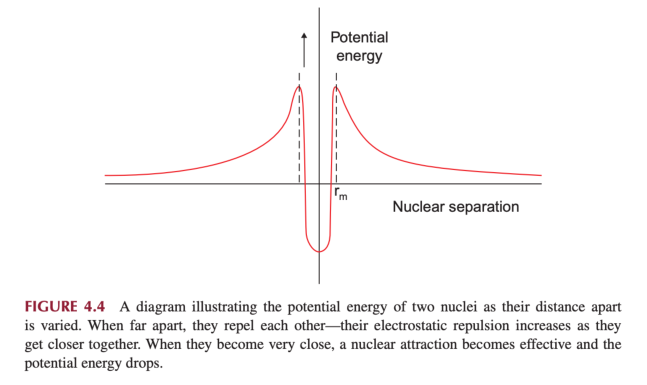
\includegraphics[width=0.65\textwidth]{chapters/fig/4_coulomb.png}
    \caption{Coulomb Barrier}
    \label{fig:4_coulomb_barrier}
\end{figure}
}

\subsection{What temperatures are needed for thermonuclear fusion? Explain with regard to the reaction cross-section.}
\solutionblock{
    The D-T reaction has the highest cross section at about 100 keV. The cross section gives the probability of a reaction to occur. The higher the cross section the higher the probability. Each reaction has a characteristic cross section curve which peaks at a certain energy. The D-T reaction requires the lowest temperature to achieve fusion.\\
    \begin{figure}[H]
        \centering
        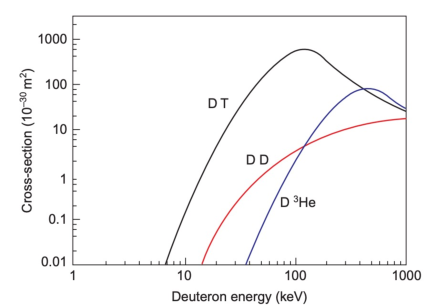
\includegraphics[width=0.65\textwidth]{chapters/fig/4_cross_section.png}
        \caption{Cross Section for different reactions}
        \label{fig:4_cross_section}
    \end{figure}
}

\subsection{Explain the power amplification factor, break-even point, and ignition criterion.}
\solutionblock{
\textbf{Power amplification factor: } A fusion energy gain factor, usually expressed with the symbol $Q$, is the ratio of fusion power produced in a nuclear fusion reactor to the power required to maintain the plasma in steady state. There are two break-even points: \textbf{engineering break-even} which is the point where the fusion power equals the heating power and \textbf{economic break-even} which is the point where the fusion power equals the heating power plus the power needed to produce the plasma i.e. operating costs of the plant.\\
Self heating of the plasma is only achieved when the gain factor is $Q\approx5$.\\
\textbf{Ignition criterion: } Ignition is the point where the fusion power produced is higher than the heating power. This is the point where the plasma is self-heating (menaing $Q \approx 5$).\\
}

\subsection{What is the fusion triple-product? Explain all three terms and the ways to get a high value in magnetic and inertial confinement fusion.}
\begin{multisolutionblock}
The triple product is a figure of merit used in fusion research. It is the product of the plasma density $n$, the plasma temperature $T$ and the energy confinement time $\tau_E$.\\
\begin{equation}
    nT\tau_E > 3 \cdot 10^{21} m^{-3}keV \, s
\end{equation}
\begin{figure}[H]
    \centering
    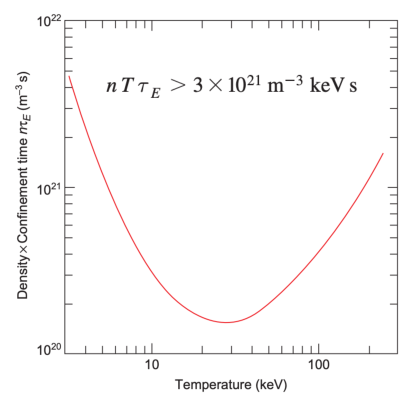
\includegraphics[width=0.65\textwidth]{chapters/fig/4_triple_product.png}
    \caption{The ignition criterion: the value of the product of density and confinement time $n\tau_E$, necessary to obtain plasma ignition, plotted as a function of plasma temperature $T$ (on x-axis). The curve has a minimum at about $T = 30 \,keV$ (roughly $300$ million K).}
    \label{fig:4_triple_product}
\end{figure}

For the two different types of confinement we can achieve a high triple product in different ways. For magnetic confinement we can achieve a somewhat high confinement time at a lower preasure. For inertial confinement we can achieve a high pressure at a lower confinement time.\\
For both cases a temperature $T$ of about 20-30 keV is required. A $Q$ of about 5, which is needed for ignition may be achieved using magnetic confinement at 5 bars for 1 second or inertial confinement at 5 billion bars for 1 nanosecond.\\
\begin{figure}[H]
    \centering
    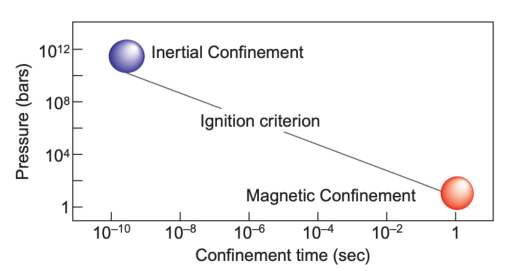
\includegraphics[width=0.65\textwidth]{chapters/fig/4_inertial_vs_magnetic.png}
    \caption{The conditions required for fusion plotted in terms of plasma pressure (bars) against confinement time (in seconds).}
    \label{fig:4_inertial_vs_magnetic}
\end{figure}
\end{multisolutionblock}

\subsection{Discuss from a historical perspective how close we are to reach scientific and technical break-even and ignition for various fusion technologies.}
\solutionblock{From an engineering standpoint we are just now able to produce magnetic confinement devices that can achieve a high enough triple product to reach ignition. However, we are still far of when it comes to ignition an thus self heating. The constant of fusion research is that we are always 30 years away from a working fusion reactor.\\
Actually we are getting closer: recent experiments at the National Ignition Facility (NIF) in the US have achieved a triple product of $Q = 1.54$ which is a factor of about 3 shy of the ignition criterion.\\
For magnetic confinement the record is held by the Joint European Torus (JET) in the UK with a triple product of $Q = 0.67$. For $Q_{ext}$ (only measuring the energy input from external sources) the record stands at $Q_{ext} = 1.25$ slightly besting JET's $Q_{ext}$ of $1.14$.\\
}
